\documentclass[12pt]{report}
\usepackage[spanish]{babel}
\usepackage[utf8]{inputenc}
\usepackage{graphicx}
\usepackage{verbatim}
\usepackage{listings}
\usepackage{float}
\renewcommand*\thesection{\arabic{section}}

\begin{document}
	
	\begin{center}
		\textbf{Análisis de Algoritmos, Sem: 2018-1, 3CV1, Práctica 10, 12-2017}
		\newline
	\end{center}
	
	\begin{center}
		\begin{picture}(0,0) \put(-125,-55){
			\includegraphics[width=2.7cm]{../../IPNlogo.jpg}} 
		\end{picture}
		\LARGE Escuela Superior de Cómputo.\\
		Instituto Politécnico Nacional, México.\\
		\begin{picture}(0,0) \put(160,10){
			\includegraphics[width=2.7cm]{../../logoescom.png}} 
		\end{picture}
	\end{center}
	
	\begin{center}
		\Large Práctica 10: Verificación en Tiempo Polinomial.\\
	\end{center}
	
	\begin{center}
		\textbf{Blancas Pérez Bryan Israel}\\
		orionmunecaycanica@gmail.com\\
	\end{center}
	
	
	\textbf{\large Resumen: }Implementar un algoritmo que verifique un grafo $C$ , para determinar si es o no un ciclo Hamiltoniano de un grafo $G$, además de mostrar que este algoritmo, se ejecuta en tiempo polinomial. \newline\\
	\textbf{\large Palabras Clave: } Ciclo Hamiltoniano, Grafo Hamiltoniano, Verificación en Tiempo Polinomial, Complejidad Computacional, Problemas NP y NP-completos.\\
	

	\section{Introducción}
	\textbf{Verificación en Tiempo Polinomal.}\\
	En la Teoría de la Complejidad Computacional, se sabe que para resolver problemas pertenecientes a la clase de complejidad NP, se requiere de una Máquina de Turing no Determinista, ya que con la tecnología actual, el tiempo necesario para encontrar la solución de estos problemas es super-polinomal. Por el contrario, para los problemas que pertenecen a la clase de complejidad P, es posible hallarles una solución en tiempo polinomial. Sin embargo, una propiedad de los problemas NP, es que se puede verificar si una propuesta de solución lo es realmente, implementando un algoritmo que se ejecute en tiempo  polinimial. Este artículo, pretende mostrar lo anterior dicho, verificando una solución para el problema del ciclo Hamiltoniano, problema que se sabe es NP-completo.
	
	\newpage

	\section{Conceptos Básicos}
	\textbf{Problema del Ciclo Hamiltoniano.}\\
	
	En teoría de grafos, el problema del ciclo Hamiltoniano trata de determinar si un ciclo Hamiltoniano existe o no en un determinado grafo. Se sabe que este problema pertenece a la clase NP-completo, lo cual nos dice que aún no se encuentra un algoritmo polinomial que halle la solución.[1]\\
	En esta práctica, se pretende demostrar una propiedad de los problemas de la clase NP-completos, la cual es verificar si una propuesta de solución dada, lo es o no para el problema del ciclo Hamiltoniano.
	\newline
	
	\textbf{Ciclo Hamiltoniano.}\\
	
	Un ciclo Hamiltoniano, es un camino de un grafo (sucesión de aristas adyacentes), que visita todos los vértices del grafo una y sólo una vez, si además el último vértice visitado es adyacente al primero.[2]\\
	En la figura 1, se muestra un ejemplo de un ciclo Hamiltoniano en un grafo arbitrario.
		
		\begin{figure}[H]
			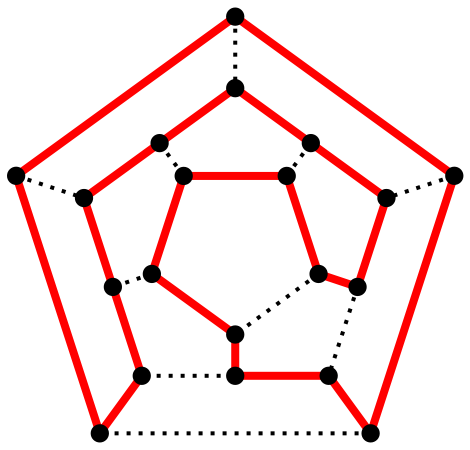
\includegraphics[height=6cm]{imagenes/1.png}
			\centering
			\caption{Ciclo Hamiltoniano.}
			\centering
		\end{figure}
	
	
		

	\section{Experimentación y Resultados}	
	\textbf{Ejercicio 1.}\\
Implementar un algoritmo para verificar el problema de los ciclos Hamiltonianos, es
decir, implementar un algoritmo \textbf{Verificacion\_Hamilton(Grafo G, certificado C)} que verifique en tiempo polinomial (muestre esto mediante gráficas y analíticamente) que el certificado $C$ es o no un ciclo Hamiltoniano del grafo $G$.\\

Pseudocódigo del algoritmo:
\lstset{language=python, breaklines=true, basicstyle=\footnotesize}
\lstset{numbers=left, numberstyle=\tiny, stepnumber=1, numbersep=10pt}
\begin{lstlisting}
Verificacion_Hamilton(Grafo G, Certificado C)

  #Verificar que los nodos de C, existan en G
  
  for node in C:
    if node.existIn(G)==0 :
      print "Nodo inexistente"
      return 0
     
  #Verificar que las aristas usadas en C, existan en G 
  
  for arista in C:
    if arista.existIn(G)==0:
      print "Arista Inexistente"
      return 0

  #Verificar que se visite cada nodo una vez, y que  C sea un circuito
  
  frecuencia_nodos[NodesIn(G)][2]
  
  for i=0 to NodesIn(G):
      frecuencia_nodos[i][1]=0
  
  i=0
  for node in G:
    frecuencia_nodos[i++][0]=node
    
  for node in C:
    k=find(frecuencia_nodo,node)
    frecuencia_nodo[k][1]++
    
  
  for i=0 to NodesIn(G):
    if(frecuencia_nodo[i][1]<1)
      print "Grafo C no es un circuito, nodo i no visitado"
      return 0
    if(frecuencia_nodo[i][1]>1)
      print "Nodo i visitado mas de una vez"
      return 0
  
  return 1
\end{lstlisting}

El algoritmo implementado, primero checa que todos los nodos de la solución $C$, existan en el grafo $G$, de lo contrario retorna 0 lo cual significa que no es solución al problema. EL siguiente paso que se realiza, es verificar que las aristas utilizadas en la solución $C$, existan en el grafo G. Y finalmente, se verifica que los nodos en la solución $C$, hayan sido visitados una y sólo una vez. Este último paso, se realiza utilizando una matriz que funciona como una tabla de frecuencia, en donde la primer columna contiene el nodo y la segunda columna contiene el número de veces que se visitó en el camino. Si la solución pasa las 3 verificaciones, el algoritmo retorna 1, lo cual significa que el certificado $C$, es en realidad un ciclo Hamiltoniano del grafo $G$. 
\\

\textbf{Ejecución del Algoritmo.}\\
	
	\textbf{Input}.\\
Formato del archivo input.txt, (Grafo $G$)	
\lstset{language=c, breaklines=true, basicstyle=\footnotesize}
\lstset{numbers=left, numberstyle=\tiny, stepnumber=1, numbersep=10pt}
\begin{lstlisting}
5	//# nodos
7	//# aristas
1 2	//aristas nodoInicio nodoFin
1 3
1 4
2 4
2 5
3 4
4 5
\end{lstlisting}
Formato del archivo solución.txt, (Certificado $G$)	
\lstset{language=c, breaklines=true, basicstyle=\footnotesize}
\lstset{numbers=left, numberstyle=\tiny, stepnumber=1, numbersep=10pt}
\begin{lstlisting}
5	//# aristas
1 2	//aristas nodoInicio nodoFin
2 5
5 4
4 3
3 1
\end{lstlisting}
\newpage

Las figuras 2 y 3, muestran la interpretación de los archivos de entrada.

	\begin{figure}[H]
		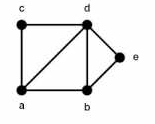
\includegraphics[height=6cm]{imagenes/2.png}
		\centering
		\caption{Interpretación de input.txt.}
		\centering
	\end{figure}
	
	\begin{figure}[H]
		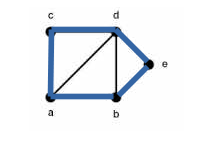
\includegraphics[height=6.5cm]{imagenes/3.png}
		\centering
		\caption{Interpretación de solución.txt.}
		\centering
	\end{figure}
	
	\newpage
\textbf{Output.}
	\begin{figure}[H]
		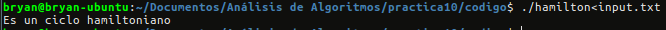
\includegraphics[width=16cm]{imagenes/4.png}
		\centering
		\caption{Output.}
		\centering
	\end{figure}
	
	Si cambiamos solución.txt a:
	\lstset{language=c, breaklines=true, basicstyle=\footnotesize}
	\lstset{numbers=left, numberstyle=\tiny, stepnumber=1, numbersep=10pt}
	\begin{lstlisting}
	5	
	1 2	
	2 5
	5 4
	4 3
	3 5
	\end{lstlisting}

	\begin{figure}[H]
		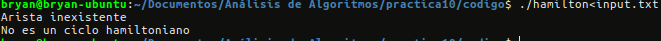
\includegraphics[width=16cm]{imagenes/5.png}
		\centering
		\caption{Output 2.}
		\centering
	\end{figure}
	
	\textbf{Demostración analítica del orden de complejidad de la verificación.}\\
	
	Orden de complejidad por verificación realizada (ver pseudocódigo página 3).\\
	Sea $nC$ y $aC$ el número de nodos y de aristas respectivamente en el certificado $C$.\\
	Sea $nG$ y $aG$ el número de nodos y de aristas respectivamente en el grafo $G$.\\
	Verificación 1: $O(nC)$\\
	Verificación 2: $O(aC)$\\
	Verificación 3: $O(nC*nG)$\\
	
	Como las verificaciones están en el mismo nivel, se concluye que el algoritmo tiene un orden de complejidad $O(nC*nG)$, pero para poder ser un ciclo Hamiltoniano es necesario que los nodos usados en el certificado $C$, sean los mismos que existen en el grafo $G$, entonces $nC=nG=n$.
	
	$Por \ lo \ tanto \ verificacionHamilton \ \epsilon \ O(n^2).$
	
	\newpage
	\textbf{Demostración mediante gráficas del orden de complejidad de la verificación.}\\
	
	La figura 6, muestra la gráfica $T(n) \ vs \ n$, del algoritmo de verificación de los ciclos Hamiltonianos. La función roja, es $T(n)=n^{2}$, mientras que los puntos son los datos obtenidos de la ejecución del algoritmo, demostrando así, que el algoritmo tiene orden de complejidad $\O(n^2)$, y más aún demostrando que el algoritmo se ejecuta en tiempo polinomial.\\
	
	\begin{figure}[H]
		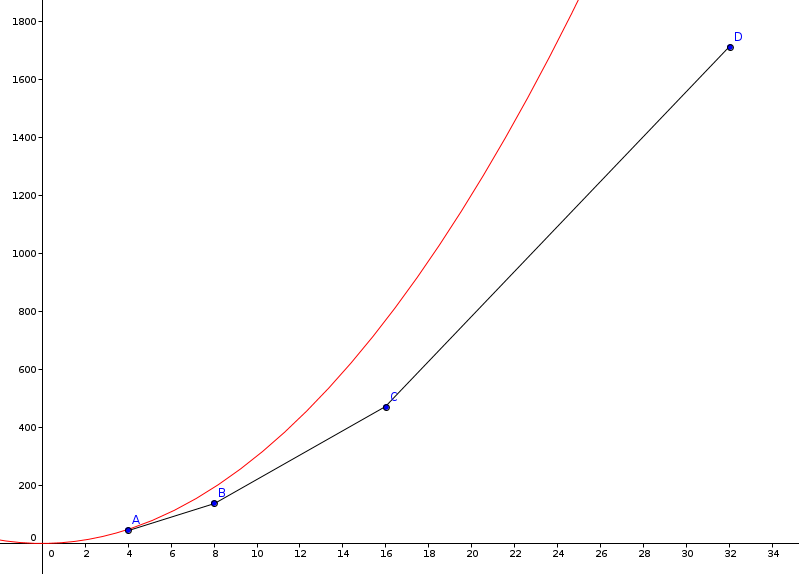
\includegraphics[width=14.7cm]{imagenes/output.png}
		\centering
		\caption{Output.}
		\centering
	\end{figure}
	  
\newpage		
\section{Conclusiones}
Esta práctica es muy útil para demostrar que los problemas NP pueden verificarse en tiempo polinomial, pero a su vez nos da una perspectiva de lo difícil que es resolverlos. Tuve problemas al demostrar el orden de complejidad de manera analítica, sin embargo después de mucho analizar, pude dar con el resultado. También se me complico la implementación del algoritmo planteado, puesto que se tenían que hacer muchos ajustes para implementarlo en un lenguaje de programación como C.\\
A mi parecer esta última práctica termina con un muy buen curso en donde las prácticas definitivamente han sido lo mejor de éste.

\newpage

\section{Bibliografía}

[1] https://es.wikipedia.org/wiki/Problema\_del\_ciclo\_hamiltoniano\\

[2] https://es.wikipedia.org/wiki/Camino\_hamiltoniano\\
	
	
\end{document}